\begin{inhalt}
\renewcommand*\chapterpagestyle{scrheadings}

\section{Parameter}

Anhand von Online-Recherche \cite{Luftparameter1, Luftparameter2} wurden folgende Parameter für die Luftqualitätsmessung festgelegt:

\begin{itemize}
    \item \textbf{Temperatur}
    \item \textbf{Luftfeuchtigkeit}
    \item \textbf{CO$_2$}
    \item \textbf{VOC}
\end{itemize}

CO$_2$ und VOCs, sind in Innenräumen die relevantesten Schadstoffe. 

\smallskip

Kohlenstoffdioxid oder Kohlendioxid (CO$_2$) ist eine chemische Verbindung aus Kohlenstoff und Sauerstoff. CO$_2$ ist ein nicht brennbares, saures und farbloses Gas. Es entsteht unter anderem durch Verbrennung oder durch Ausatmung. \cite{CO2Wiki}

\smallskip

Luftschadstoffe werden kurz als VOC bezeichnet. Die Abkürzung VOC (Volatile Organic Compounds) steht für flüchtige organische Verbindungen. Es handelt sich dabei um organisch-chemische Verbindungen des Siedebereiches von ca. 50 – 260°C. VOC sind praktisch jederzeit und überall in der Raumluft enthalten. \cite{Luftparameter1}


\section{Komponenten}

\subsection{Mikrocontroller}

Da in dieser Diplomarbeit darauf geachtet wurde, hauptsächlich Komponenten mit europäischer Herkunft zu verwenden, fiel die Wahl des Mikrocontrollers auf den Pico W der Raspberry Pi Foundation. Dieser basiert auf dem RP2040-Mikrocontroller und unterstützt MicroPython sowie C/C++. Der Raspberry Pi Pico W ist mit einem WLAN-Modul ausgestattet und besitzt Interfaces für SPI und I2C, welche für diese Diplomarbeit benötigt werden. \cite{Raspberry_Pi_Pico_W}

\subsection{Sensoren}

\textbf{CO$_2$-Sensor:}

\smallskip

Der PASCO2V01 ist ein CO$_2$-Sensor der Marke Infineon (Österreich). Der Sensor misst den CO$_2$-Anteil in der Luft in PPM (Parts Per Million). Er benötigt 3,3V sowie 12V als Spannungsversorgungen und kann unter anderem mit I2C angesteuert und ausgelesen werden. \cite{PASCO2V01}

Benutzt wird das Mini Evaluation Board für den XENSIV™ PAS CO2-Sensor \cite{PASCO2_Miniboard}, da es bereits integrierte Pins besitzt und deshalb kein feines SMD-Löten erforderlich ist. 
\bigskip \\

\textbf{Gas-Sensor:}

\smallskip

Der BME688 ist ein Luftqualitätssensor der Marke Bosch (Deutschland) \cite{BME688}. Er wird mittels I2C angesteuert bzw. ausgelesen. Der BME688 misst Temperatur in °C, relative Luftfeuchtigkeit in Prozent, Luftdruck in hPa und Gaswiderstand in Ohm. Der Gassensor des BME688 wurde laut Datenblatt auf folgende Gase charakterisiert:

\begin{itemize}
    \item Wasserstoffsulfid (H₂S) 
    \item Ethanol (EtOH) 
    \item Kohlenmonoxid (CO)
    \item flüchtige organische Verbindungen (VOCs)
\end{itemize}

Der Gassensor misst keine einzelnen Gaskonzentrationen, sondern ermittelt einen Gaswiderstandswert. Mit diesem kann die Qualität der Luft eingeschätzt werden. \cite{BME688}
\smallskip

Benutzt wird der Environment 3 Click der Marke MIKROE (Serbien) \cite{ENVIRONMENT_3_CLICK}. Dieser basiert auf dem BME688 von Bosch und besitzt integrierte Pins sowie Auswahlmöglichkeiten für die Adresse und das Bussystem (Kap. \ref{sec:Pin_Zuordnungen}), direkt am Board.

\subsection{Display}

Damit die gemessenen Parameter auch direkt am Gerät abgelesen werden können, wurde ein Display miteingebunden. Da kein touchscreenfähiges Display vorgesehen war, wurde das 2 Zoll-LCD-Modul von Waveshare gewählt. Dies ist ein 320 × 240 Pixel LCD-Display, welches über SPI angesteuert wird und eine Gesamtgröße von 58mm × 35mm aufweist. \cite{LCDDisplayWiki}

\subsection{Benutzer Interaktion} \label{sec:Benutzer_Interaktionen}

Damit der Benutzer mit dem Gerät interagieren kann, wurden zwei Taster miteingebunden. Mithilfe dieser kann der Benutzer zwischen den unterschiedlichen Seiten des Displays wechseln und verschiedene Einstellmöglichkeiten vornehmen (Kap. \ref{sec:display interface}).

\subsection{USB4125 / USB4175} \label{sec:USB4125_75}

USB4125 und USB4175, sind USB-Typ-C-Buchsen von GCT (Global Connector Technology), die speziell für Ladeanwendungen entwickelt wurden und ausschließlich Strom übertragen, ohne Datenleitungen. \cite{USB4125}, \cite{USB4175}

\section{Display Interface} \label{sec:display interface}

Als Designidee für das Display-Layout wurden Skizzen mit Excalidraw \cite{Excalidraw} entworfen. Das Display soll verschiedene Seiten aufweisen, zwischen denen mit Tastern gewechselt werden kann. 

\smallskip

\begin{center}
    \textbf{Seite 1:}
\end{center}

\begin{figure}[!htb]
\centering
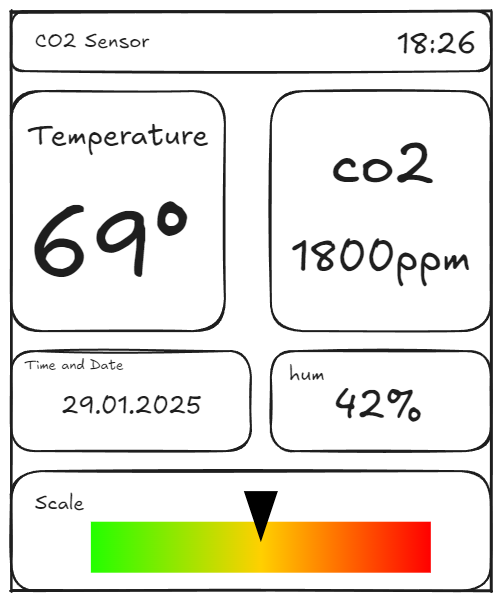
\includegraphics[width=0.35\textwidth]{files/Tobias/pics/Skizzen/Screen1_Sensor_Info.png}
\caption[Display Interface Skizze (Seite 1)]{}
\label{fig:display_skizze_seite_1}
\end{figure}

Am oberen Rand befindet sich die Seitenbezeichnung („CO2-Sensor“) sowie die aktuelle Uhrzeit in einem schmalen Feld. Darunter werden die Messwerte CO2 und Temperatur in größeren Feldern angezeigt, während sich das aktuelle Datum und die Luftfeuchtigkeit in kleineren Feldern darunter befinden. Ganz unten zeigt eine Skala die Luftqualität anhand des gemessenen Gaswiderstands an. Die Skala verläuft von Grün (gute Qualität) bis Rot (schlechte Qualität), und durch einen Zeiger wird der aktuelle Zustand markiert.

\begin{center}
    \textbf{Seite 2:}
\end{center}

\begin{figure}[!htb]
\centering
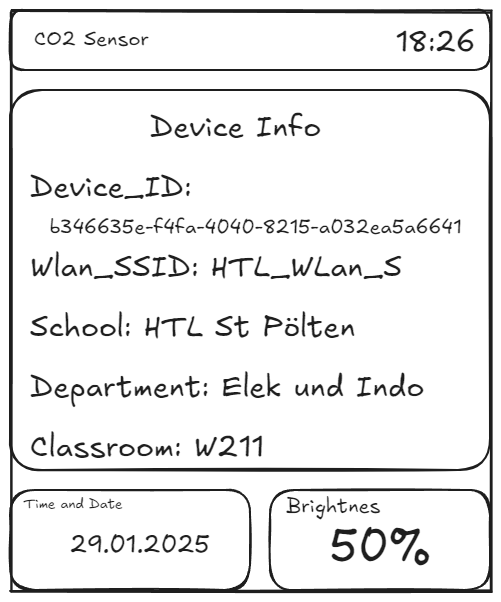
\includegraphics[width=0.35\textwidth]{files/Tobias/pics/Skizzen/Screen2_Info.png}
\caption[Display Interface Skizze (Seite 2)]{}
\label{fig:display_skizze_seite_2}
\end{figure}

Diese Seite der Benutzeroberfläche stellt Informationen über das Gerät bereit. Am oberen Rand befindet sich die Seitenbezeichnung sowie die aktuelle Uhrzeit. Direkt unter der Überschrift befindet sich eine große rechteckige Box mit der Überschrift „Device Info“. Innerhalb dieses Felds sind verschiedene Informationen aufgelistet:
\begin{itemize}
    \item Device ID
    \item WLAN-SSID
    \item School
    \item Department
    \item Classroom
\end{itemize}

Am unteren Ende der Seite befinden sich zwei Felder mit dem aktuellen Datum und der Helligkeitsstufe des Displays in Prozent.

\begin{center}
    \textbf{Seite 3:}
\end{center}

\begin{figure}[!htb]
\centering
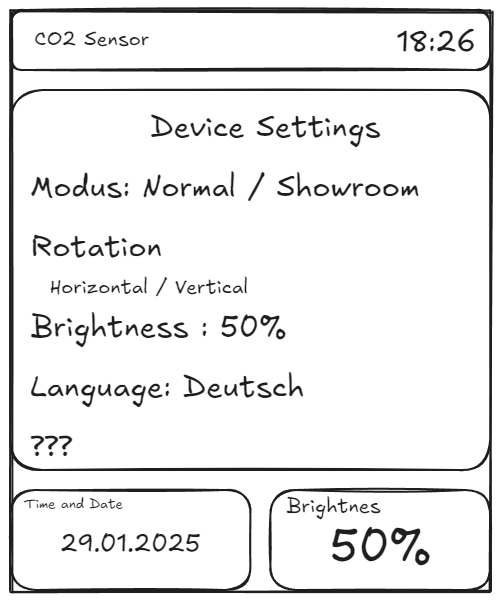
\includegraphics[width=0.35\textwidth]{files/Tobias/pics/Skizzen/Screen3_Settings.png}
\caption[Display Interface Skizze (Seite 3)]{}
\label{fig:display_skizze_seite_3}
\end{figure}

Die dritte Seite zeigt die Konfiguration des Geräts. Der Aufbau ähnelt den anderen Seiten: oben die Seitenbezeichnung und Uhrzeit, darunter eine große Box mit den Hauptinhalten. Hier können verschiedene Einstellungen vorgenommen werden:

\begin{itemize}
    \item Modus („Normal“ oder „Showroom“)
    \item Display-Ausrichtung (horizontal oder vertikal)
    \item Helligkeit
\end{itemize}

Zusätzliche Markierungen („???“) deuten an, dass noch weitere Einstellungsoptionen ergänzt werden können.

\begin{center}
    \textbf{Showroom:}
\end{center}

\begin{figure}[!htb]
\centering
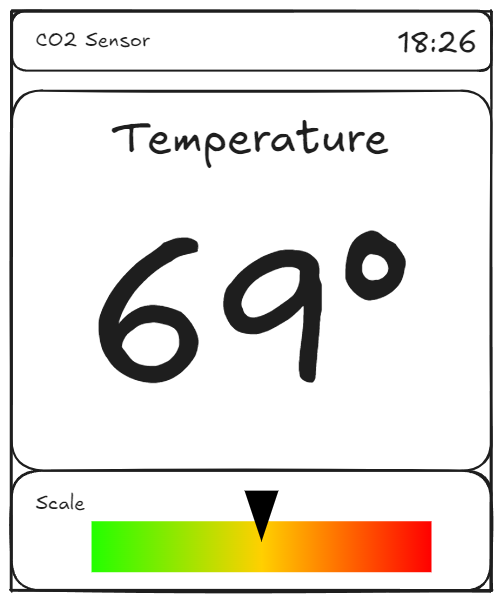
\includegraphics[width=0.35\textwidth]{files/Tobias/pics/Skizzen/Showroom1.png}
\caption[Display Interface Skizze (Showroom)]{}
\label{fig:display_skizze_showroom1}
\end{figure}

Der oben erwähnte Showroom ist ein Modus, in dem nicht eine fixe Seite angezeigt wird, sondern zwischen verschiedenen Seiten gewechselt wird. Der Sinn dahinter ist, die gemessenen Parameter einzeln und groß auf der Seite darzustellen. Dabei wird automatisch zwischen den Parametern gewechselt. Das obere Feld mit der Seitenbezeichnung und Uhrzeit sowie das untere Feld mit der Skala bleiben erhalten.

\end{inhalt}